\section*{Annexes}


\begin{figure}[!ht]
  \center{
    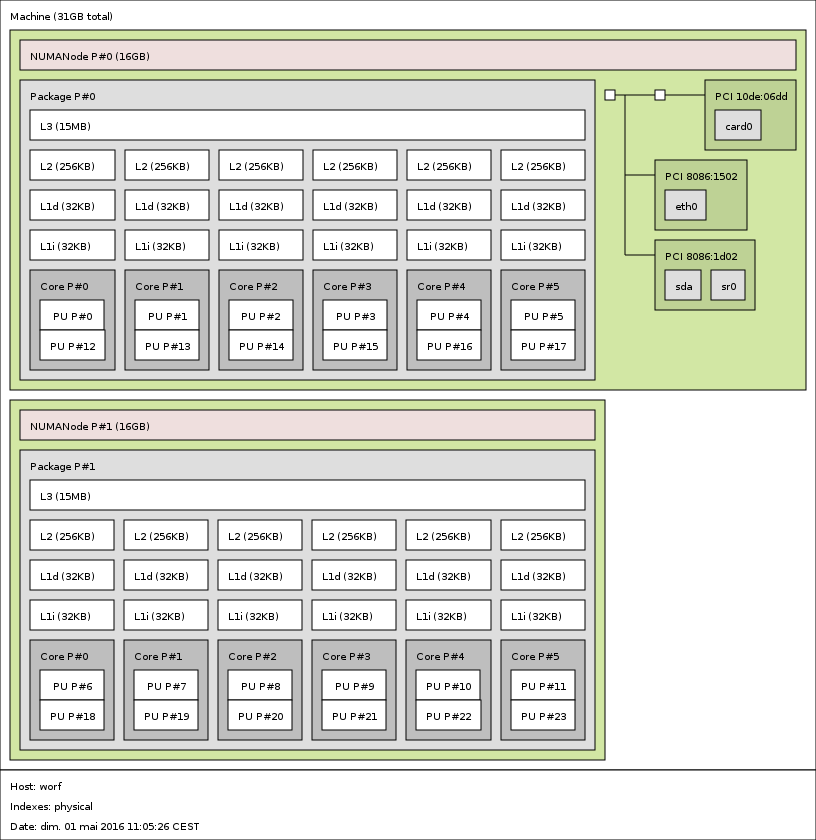
\includegraphics[width=17cm]{images/proc.png}
  }
  \caption{Configuration de la machine hôte \texttt{worf}.}
  \label{fig:lstopo}
\end{figure}

\clearpage
\subsection*{Algorithmes}

\subsubsection*{Version séquentielle de référence}
\label{algo:naif}

\begin{verbatim}
void compute_naive (sand_t sand)
{
  int change = 0;
  do {
    for (int y = 1; y < DIM-1; y++){
      for (int x = 1; x < DIM-1; x++)
	if(sand[y][x] >= 4) {
	  change = 1;
	  sand[y][x] -= 4;
	  sand[y-1][x] += 1;
	  sand[y+1][x] += 1;
	  sand[y][x-1] += 1;
	  sand[y][x+1] += 1;
	}
    }
  }
  while(change);
}
\end{verbatim}
